%----------------------------------------------------------------------------------------
%	PAQUETES Y OTRAS COSAS DE CONFIGURACION
%----------------------------------------------------------------------------------------
%\documentclass[a4paper,man,natbib,scrbook]{apa6}
\documentclass[12pt]{article}

% esto es una prueba de comment
\usepackage[spanish]{babel}
\usepackage[utf8x]{inputenc}
\usepackage{graphicx}
%\usepackage[colorinlistoftodos]{todonotes} %PAQUETE QUE FALLA JULIO
\usepackage[bottom]{footmisc}
%\usepackage{blindtext} %PAQUETE QUE FALLA JULIO
\usepackage{caption}
\graphicspath{ {images/} }
%\graphicspath{{/home/cursoredes/images/}}
\usepackage{fancyhdr}
\usepackage{enumitem}
\usepackage{hyperref} %INDICE CON VINCULOS
\usepackage{csquotes}
%\usepackage{mdframed}


%----------------------------------------------------------------------------------------
%	PAGE HEADERS
%----------------------------------------------------------------------------------------
\setlength{\headheight}{15pt}

\pagestyle{fancy}
\renewcommand{\sectionmark}[1]{ \markright{#1} }

% L=left, R=right, E=even, O=odd

\fancyhf{}
\fancyhead[LE,RO]{\thepage} %Numero pagina
\fancyhead[RE]{\textit{ \nouppercase{\leftmark}} }
\fancyhead[LO]{\textit{ \nouppercase{\rightmark}} }

\fancypagestyle{plain}{ 
  \fancyhf{} 
  \renewcommand{\headrulewidth}{0pt} 
  \renewcommand{\footrulewidth}{0pt}
}
%------------------------------------------------
%
%------------------------------------------------

\begin{document}

\begin{titlepage}

\newcommand{\HRule}{\rule{\linewidth}{0.5mm}} 

\center % Centra todo
 
 
%----------------------------------------------------------------------------------------
%	LOGO SECCION
%----------------------------------------------------------------------------------------

\textsc{\LARGE Universidad Complutense de Madrid}\\[0.1cm] % Universidad

\begin{center}
	\centering
	
\includegraphics[width=0.5\textwidth]{logo}
\end{center}
 
 
%----------------------------------------------------------------------------------------
%	HEADING SECCION
%----------------------------------------------------------------------------------------

\textsc{\LARGE Grupo 4}\\[0.1cm] % Grupo
%\textsc{\Large Heading 1}\\[0.\\5cm] % Heading mayor
%\textsc{\large Heading 2}\\[0.\\5cm] % Heading menor

%\textsc{\LARGE Grupo 4}\\[1cm]

%----------------------------------------------------------------------------------------
%	TITULO SECCION
%----------------------------------------------------------------------------------------

\HRule \\[0.4cm]
{ \huge \bfseries HITO 1: }\\[0.4cm] % Titulo
{ \huge \bfseries INVESTIGACIÓN }\\[0.2cm] % Titulo
\HRule \\[1.2cm]
 
%----------------------------------------------------------------------------------------
%	AUTHOR SECTION
%----------------------------------------------------------------------------------------

\begin{minipage}{0.4\textwidth}
\begin{flushleft} \large
\emph{Autores:}\\
Ángel \textsc{Cruz} \\ %Nombres
Julio \textsc{de la Cruz} \\
Eduardo \textsc{Alcober}\\
Sergio \textsc{Gómez}\\
Isauro \textsc{López}\\
Darío \textsc{Gallegos}
\end{flushleft}
\end{minipage}
\begin{minipage}{0.4\textwidth}
\begin{flushright} \large
\emph{Profesor:} \\
Antonio \textsc{Sánchez} % NOMBRE PROFESOR
\end{flushright}
\end{minipage}\\[0.66cm]
%----------------------------------------------------------------------------------------
%	FECHA SECCION
%----------------------------------------------------------------------------------------
%{\large 2 de diciembre de 2018}\\[0.\\5cm] % Fecha

%---------------------------------------------------------------------------------------
%	CONTENIDO
%----------------------------------------------------------------------------------------

\vfill % Rellenar el resto con espacio en blanco

\end{titlepage}


%\maketitle
%\footnotetext{EJEMPLO DE NOTA A PIE DE PAGINA}

\tableofcontents % Indice de contenidos
\newpage

\section{Introducción}
Nuestra aplicación está enfocada a cubrir las necesidades del personal de la Biblioteca María Zambrano y a los estudiantes que le dan uso.\\
\\
\\
Nuestro objetivo principal se puede resumir en la siguiente frase:
“desarrollar una aplicación que mejore la experiencia de uso de la biblioteca”.\\
\\
\\
Para llevar esta idea a cabo, debemos conocer a nuestros futuros usuarios, aprender de sus necesidades, expectativas y construir el diseño en base a ellas.\\ Los resultados de esta investigación definirán tanto el desarrollo como el producto final.\\ Esta fase posee es de gran importancia pues en función de los resultados obtenidos se desarrollará las sucesivas fases, y es que, los factoides generados ahora, determinarán nuestro margen de evolución a lo largo del diseño de nuestra idea.\\
\\
\\
Para completar esta fase de investigación, cumpliendo las fechas, realizaremos un reparto de tareas y recursos.\\ 
\section{Enfoque inicial}
Antes de empezar a realizar las entrevistas y cuestionarios a los posibles candidatos necesitábamos tener una idea básica de a quién iría dirigida nuestra aplicación.\\ En primer lugar, se habló de cinco tipos de usuarios:
\begin{itemize}

\item \textbf{Estudiantes}: Aquellos que asisten a estudiar en la biblioteca.\\
\item \textbf{Personal}: Son los trabajadores de la biblioteca.\\
\item \textbf{Docentes}: Aquellos profesores que acuden a la biblioteca.\\
\item \textbf{Particulares}: No son estudiantes de la UCM, pero van a la biblioteca.\\
\item \textbf{Erasmus}: Estudiantes extranjeros que usan la biblioteca.\\

\end{itemize}
Al final hemos decido acotar el número de usuarios para centrarnos en los más importantes: estudiantes, Erasmus y el personal.\\
\section{Reparto de tareas}
Hemos decidido distribuir la etapa de investigación en tres fases:
\begin{center}
	\centering
	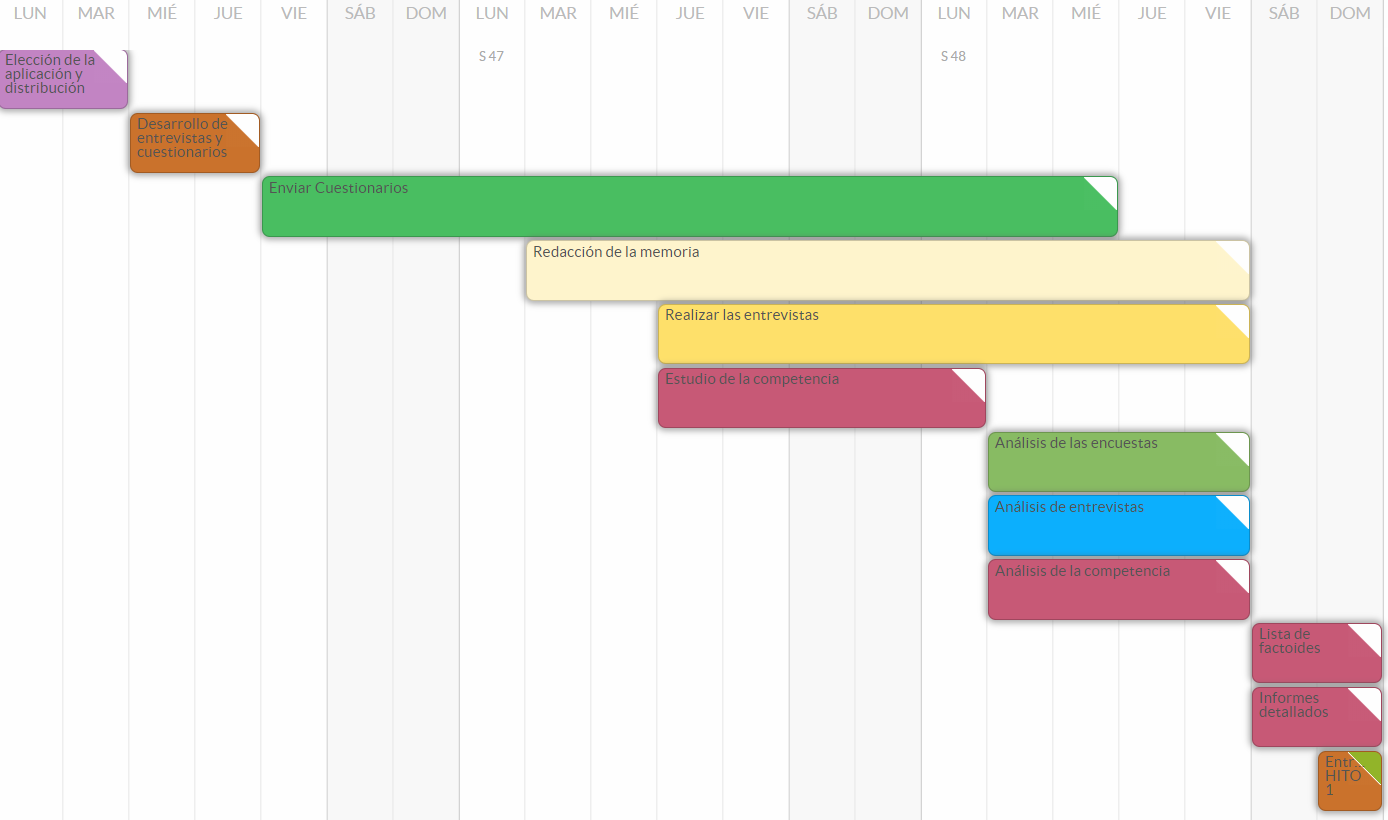
\includegraphics[width=1\textwidth]{planificacionHito1}
	\captionof{figure}{Planificación}
\end{center}
\subsection{Primera Fase}
La primera actividad es hacer un Screener que nos permita encontrar a los posibles candidatos de las entrevistas.\\ El objetivo es hallar la mayor diversidad posible en cuanto a los participantes se refiere.\\
\\
\\
	Una vez terminada la primera fase, dedicaremos todos los recursos a generar los guiones para las entrevistas y cuestionarios.\\ Los guiones serán una base para realizar las entrevistas, y será decisión del entrevistador seguirlo tal cual o hacer modificaciones a medida que se desarrolle la conversación.\\ El cuestionario es una herramienta para obtener información.\\ Nos permitirá realizar un análisis estadístico complementado la información de las entrevistas.\\ 
\\
\\
	Aproximadamente nos llevará cuatro días.\\
\subsection{Segunda Fase}
La etapa principal del hito, y en la que invertiremos más tiempo.\\ En ella se realizará la redacción del documento, envío masivo de los cuestionarios y grabación de las entrevistas.\\
\\
\\
Hemos repartido el trabajo de la siguiente manera.\\ La mitad del equipo se dedicará a realizar la documentación de la memoria y la otra mitad se ocupará de realizar las entrevistas.\\ Los cuestionarios se enviarán conjuntamente.\\ Al ser ocho miembros en el equipo se ha acordado realizar de seis y ocho entrevistas.\\
\\
\\
El resto de tareas como el plan de investigación, el estudio y el análisis de la competencia serán asignados por preferencia intentado que todos los miembros tengan la misma carga de trabajo.\\
\\
\\
En paralelo se ha iniciado un plan de investigación para conocer las ofertas del mercado, la posible competencia y el alcance de la aplicación.\\ Los escenarios para el estudio de la competencia serán la web y las apps móviles.\\
\\
\\
El tiempo de duración será de unos doce días.\\
\subsection{Tercera Fase}
Analizar la información y formalizar es la principal actividad de la esta fase.\\ El objetivo es obtener resultados detallados del análisis, resultados visuales como gráficos y la lista de factoides.\\ Trabajaremos en ella hasta el día de la entrega del hito.\\

\section{Entrevistas de usuarios}
Para el proceso de recopilación de información relevante para la creación de nuestra aplicación, por medio del grupo decidimos incluir un proceso de entrevistas a usuarios de la biblioteca.\\ Después de generar una plantilla que acompañe dichas entrevistas, conseguimos seleccionar candidatos obtenidos tanto conocidas como desconocidas al entorno del grupo.\\
\\
\\
El objetivo principal fue la motivación de acotar a los posibles candidatos, ya que los mismos fueron muy receptivos por los fines que tiene la aplicación.\\ 
\\
\\
Los candidatos seleccionados podrían pertenecer a tres tipos de usuario: estudiantes UCM, estudiantes Erasmus y personal de la biblioteca.\\ Para asegurar la obtención de información útil, decidimos crear un guion principal que pudiese servir en las entrevistas en grupo o individual y así pudiésemos interpretar dicho guion en relación de las respuestas de los entrevistados.\\
\\
\\
El guion contiene un párrafo legal que incluiríamos en las próximas entrevistas con el objetivo de respetar los datos de carácter personal en las mismas.\\
\newpage
\textbf{Consentimiento Legal:}
\\
%\begin{mdframed}
         Estamos trabajando en el desarrollo de una aplicación con el objetivo de ayudar a mejorar la reserva y agilización de las mesas/puestos en la biblioteca María Zambrano.
             El contenido de esta entrevista y la información resultante de la misma, será usado solo con fines académicos.\\
             Nos comprometemos a no difundir dicho contenido. 
[NOMBRE] ¿aceptas ser grabado/a en esta entrevista?
%\end{mdframed}

\subsection{Screener previo}

¿Qué edad tienes?
Esta pregunta la hacemos por enfocar el tipo de preguntas según el rango de edad 
¿Qué ocupación tienes?
Esta pregunta la hacemos para saber si es estudiante o trabajador de la biblioteca 
¿Has ido alguna vez a la Biblioteca María Zambrano?
Esta pregunta la hacemos porque necesitamos a gente que tiene que ir
Si es estudiantes, ¿qué carrera está realizando?
Para tener un bloque de estudiantes de distintas carreras, si es posible
¿Perteneces a la Universidad Complutense de Madrid?
Esta pregunta la hacemos porque en periodo de exámenes solamente puede entrar gente con carnet de la UCM



\subsection{Guion de entrevistas}

[[Preguntas sobre esa persona (técnicos/trabajadores de la M.\\ Zambrano)]] 

1.\\ ¿Cuánto tiempo llevas trabajando en la María Zambrano? 
2.\\ ¿Has estado trabajando en otro lugar (biblioteca…)? 
3.\\ ¿Cuáles son los problemas que son más frecuentes en la biblioteca? 
4.\\ ¿Has tenido algún problema con el alquiler/reserva de libros? ¿Cuál fue? ¿Cómo lo solucionaste?
5.\\ ¿Has tenido problemas con la búsqueda de libros? ¿Cuál fue? ¿Cómo lo solucionaste?
6.\\ ¿Cuántas veces al mes (((o algún mes en concreto))) has visto la biblioteca saturada? (Alguna vez se ha saturado la biblioteca, en qué época, qué hacéis en esos casos y como solucionais la saturación)
7.\\ (((Si dice >=1: preguntar → Cuéntanos cuales han sido los problemas más graves con las reservas que hayas tenido)))
8.\\ ¿Qué herramienta (móvil, portátil…) te sería más rápida para controlar un servicio de reservas? ¿Qué herramientas informáticas utilizáis ahora para la gestión de la biblioteca? ¿Podrías mostrarnos la interfaz, sin información concreta? 
9.\\ ¿Sueles ver a gente yendo sola o en grupo? (((para que veamos si es totalmente necesario hacer reservas en grupo o es algo más opcional))) 
10.\\ ¿Cuánto tardas en atender/ayudar a los estudiantes que buscan mesa? ¿Cómo podría agilizarse esto? 
11.\\ ¿De las labores que desempeñas en tu puesto de trabajo habitual, cuáles crees que no podrían ser automatizadas? ¿Por qué? 
12.\\ ¿Cuánto tiempo crees que pasa cada estudiante de media en las instalaciones en periodo habitual? ¿Y en exámenes? 

[[Preguntas sobre esa persona (estudiante)]]

1.\\ ¿Cuánto llevas en la Complutense?, en el tiempo que llevas ¿ha existido problemas con escoger mesas? 
2.\\ ¿Cuántas veces al mes sueles ir a la María Zambrano? 
3.\\ Cuando vas, ¿sueles ir en grupo o individualmente? ¿con cuántas personas sueles ir? 
4.\\ ¿Cuántas horas llegas a estar allí? ¿Se te hace pesado? 
5.\\ ¿Cuáles son los problemas que son más frecuentes en la biblioteca? 
6.\\ ¿Has tenido algún problema con el alquiler/reserva de libros? ¿Cuál fue? ¿Cómo lo solucionaste? 
7.\\ ¿Has tenido problemas con la búsqueda de libros? ¿Cuál fue? ¿Cómo lo solucionaste? 
8.\\ ¿Qué servicios de la biblioteca utilizas? ¿Y cuáles con más frecuencia? 
9.\\ Descríbenos un poco cómo los utilizas, es decir, los pasos que sigues.\\ 
10.\\ ¿Alguno de estos procesos se te hace tedioso o complicado? ¿Por qué? 
11.\\ ¿Cómo piensas que podría mejorar la gestión de esto la biblioteca? 
12.\\ ¿En qué puntos de esta gestión conservarías el personal humano, y cuales crees que se pueden automatizar? ¿Qué es lo que más te gusta que algunos servicios estén aún atendidos por personas? 
13.\\ ¿Crees que algunos de estos servicios podrían ser automáticos? ¿Facilitaría esto la gestión o la empobrecería? 
14.\\ ¿Si se pudieran reservar los puestos, de cuánto tiempo harías las franjas de tiempo de uso?
15.\\ ¿Cada cuánto tomas un descanso cuando estudias? 
16.\\ En caso de saturación de la biblioteca, para buscar una igualdad de uso para todos los estudiantes, ¿cuánto debería de ser el máximo tiempo de uso por estudiante / día?
17.\\ ¿Cómo harías un sistema de reservas?: Usa tu imaginación y sé breve.\\



\subsection{Resultados de las entrevistas}

Se van han adjuntar los vídeos en esta carpeta, ya que pesan mucho (25 GB aprox.\\): [VÍDEOS DE LAS ENTREVISTAS]

Entrevista 1

La bibliotecaria de la María Zambrano como la entrevistada.\\ 
El estudiante Álvaro  más adelante como el entrevistador.\\
El estudiante Sergio más adelante como el cámara.\\
	
Vídeo 1: 
00:09 – la entrevistada nombra cuál es su trabajo en la María Zambrano.\\ 
00:34 – señala que está trabajando desde 1995 y siempre ha estado en ese puesto.\\
Vídeo 2:
[Nada relevante, está atendiendo a una persona] 
Vídeo 3:
00:29 – la entrevistada tiene quejas con la búsqueda de materiales.\\ 
00:50 – la entrevistada habla sobre el servicio CISNE y un poco la implementación de los módulos.\\ 
01:26 – la entrevistada tiene quejas sobre Millenium por falta de actualizaciones y porque la atención al cliente está solamente señalada para personas de habla inglesa.\\
02:14 – la entrevistada dice que la biblioteca no tiene un equipo informático.\\
03:17 – la entrevistada se queja de los módulos, señalando más esa semana en concreto (en la que se hace la entrevista).\\
04:09 – la entrevistada deja claro que tiene un perfil básico sobre conocimientos informáticos.\\
05:00 – la entrevistada dice que hay 3 trabajadores en la biblioteca para 1500 sitios aprox.\\
Vídeo 4: 
00:20 – la entrevistada hace una queja sobre que los “usuarios Erasmus” no pueden sacar libros.\\ 
02:23 – la entrevistada dice que recurren al programa antiguo, que no se pueden hacer cambios, pero si consultas para encontrar usuarios y documentos.\\
03:33 – la entrevistada se queja del actual software de gestión.\\
04:30-05:30 – la entrevistada tiene una manía muy extraña a los orientales.\\
05:55 – la entrevistada sigue señalando que el antiguo software (CISNE) de búsquedas daba menos problemas, y que el actual (BUCea) los duplica.\\
07:27 – la entrevistada recuerda que se le señaló al director que se pusiera antes CISNE que BUCea, pero dijo que no porque ya se había pagado.\\
Vídeo 5:
00:10 – la entrevistada recuerda que todos los módulos colgaban de CISNE y Millenium.\\
00:46 – la entrevistada dice que la gente de arriba no comunicó todos los problemas que se iban a generar.\\
Vídeo 6:
00:10 – la entrevistada cuenta una queja sobre el catálogo.\\ 
01:49 – la entrevistada se queja sobre la administración y el descontento que existe.\\
02:00 – la entrevistada muestra una pena sobre “la corrupción” existente en la UCM.\\
03:45 – la entrevistada sigue quejándose sobre la falta de compresión que se tiene sobre los usuarios desde los altos cargos y etc.\\
04:22 – el entrevistador recuerda el fallo que existe con el módulo de préstamos.\\
05:12 – la entrevistada señala la mala gestión del personal, ya que debería haber 1-2 personas de procesos técnicos.\\
Vídeo 7: 
00:55 – la entrevistada se vuelve de nuevo a quejar con el catálogo.\\
02:20 – la entrevistada dice que si se puede ver la disponibilidad de los libros, el sistema de préstamo no ha cambiado.\\
02:40 – la entrevistada dice que el módulo de reserva no se ha adaptado correctamente, ya que puedes coger un libro de una facultad y devolverlo en la María Zambrano (remarca que es un problema para ellos).\\
03:35 – la entrevistada comenta que no penaliza la devolución y que son problemas que se están ocultando de cara al público.\\
06:35 – la entrevistada deja claro que no se implementan las cosas bien y que lleva esto desde el curso pasado.\\
08:25 – la entrevistada dice que en la María Zambrano hay muchos libros perdidos de otras facultades.\\
10:35 – la entrevistada dice que no hay reserva de puestos y dice que se pidieron unos tornos para que entren solo los de la Complutense.\\
11:03 – la entrevistada comenta que si no tienen el carnet (para poder entrar) se les mira en la base de datos (proceso tedioso y lento), pero si son nuevos no aparecen en esta.\\
11:20 – la entrevistada dice que ahora el proceso para controlar a la gente es con un sello.\\
11:53 – la entrevistada comenta que las aperturas extraordinarias son las que dejan quejas importantes.\\
Vídeo 8:
00:24 – la entrevista, el entrevistador y el cámara comentan la falta de reivindicación (la falta de quejas).\\
01:09 – la entrevistada comenta algo más básico que hizo un compañero suyo para contar el aforo de la biblioteca y dice que no se mira en la María Zambrano el aforo (mucho descontrol).\\
03:57 – la entrevistada explica un poco la mala traducción del software que utilizan.\\
05:51 – la entrevistada señala los fallos del módulo, la mala interfaz.\\

Entrevista 2

Sara ha estudiado la carrera de Filología Hispánica, Español Lengua y literatura y el Máster de Español para Extranjeros.\\ Actualmente prepara Oposiciones.\\
Rocío es compañera de carrera de Sara, pero estudió el Máster de formación para el profesorado.\\ Opositó y está esperando que la llamen de interina.\\
Aunque son dos estudiantes trataremos la entrevista como una sola persona a la hora de sacar los factoides.\\ 
Sara: 
4:17 – Sara viene todas las tardes a estudiar las oposiciones, suele estudiar en grupos de 2/3 personas.\\
4:33 – Para Sara la Zambrano es la biblioteca más actualizada.\\
5:05 – A veces le molesta tener que ir de facultad en facultad buscando los libros.\\
6:03 – A ambas les gustaría poder devolver cualquier libro en cualquier facultad, pero desconocen si existe.\\
7:25 – Ambas utilizan los ordenadores: fijos y de préstamo, y están contentas con el sistema de préstamo.\\
9:30 – Cada 2 horas suelen salir a descansar.\\
12:20 – Zambrano es de Derecho y Filología y en exámenes se satura de alumnos de otras facultades.\\
14:10 – Suelen madrugar para coger sitio en la biblioteca, "esto es la guerra".\\
16:52 – Si arreglaran otras bibliotecas y ampliarán el horario se liberaría un poco la Zambrano.\\
18:50 – Ven difícil la gestión de los puestos.\\
20:20 – No suelen usar salas privadas sino zonas de estudio en grupo donde pueden hablar todos.\\
23:07 – El sistema de reservas es nuevo, lo acaban de cambiar y es sencillo y accesible.\\
Rocío:
4:17 – Rocío vive más lejos y viene menos, ya que estudia mejor en casa, con tanta gente se distrae, suele estudiar en grupos de 2/3 personas.\\
04:36 – Rocío a veces tiene problemas porque los libros no están donde deben.\\
6:03 – A ambas les gustaría poder devolver cualquier libro en cualquier facultad, pero desconocen si existe este servicio por parte de la UCM.\\
7:25 – Ambas utilizan los ordenadores: fijos y de préstamo, y están contentas con el sistema de préstamo.\\
9:30 – Cada 2 horas suelen salir a descansar.\\
12:20 – Zambrano es de Derecho y Filología y en exámenes se satura de alumnos de otras facultades.\\
14:10 – Suelen madrugar para coger sitio en la biblioteca, "esto es la guerra".\\
16:17 – La gente viene los fines de semana porque es la única que hay.\\
18:50 – Ven difícil la gestión de los puestos.\\
20:20 – No suelen usar salas privadas sino zonas de estudio en grupo donde pueden hablar todos.\\ 
23:07 – El sistema de reservas es nuevo, lo acaban de cambiar y es sencillo y accesible.\\

Entrevista 3

Génesis es una estudiante de la carrera de  derecho.\\ Actualmente está en el segundo año.\\
Acude 2/3 veces por semana a la biblioteca, en franjas generalmente de dos
0:52 –  Va a la biblioteca dos o tres veces por semana, en época de exámenes con más frecuencia.\\
1:00 –   Estudia durante dos horas y suele hacer descanso entre hora y hora.\\
1:35 – Utiliza los ordenadores de la biblioteca, aunque añade que son lentos y viejos.\\
2:35 – En exámenes la biblioteca está saturada.\\ Le toca madrugar para conseguir sitio.\\ En esta temporada suele pasar incluso sábados y domingos, todo el día.\\
3:55 – Su único modo de reservar mesa es dejar sus pertenencias en el sitio, lo que ha conllevado en otros casos robos de material personal y electrónico.\\ Actualmente no gestionan reservas, y el que llega primero es el que coge sitio.\\
11:23 – Está a favor de hacer un sistema de salas y de ordenadores.\\
13:30 – Es consciente de que el software de la biblioteca tiene fallos y ralentiza los procesos por su lentitud.\\ Existen errores entre la relación stock / ejemplares-en-la-bbdd que resultan en que a veces va a buscar un libro y no está.\\
17:00 – Piensa que un tiempo justo para hacer "slices" de uso individual de un puesto en la biblioteca sería de dos horas y media.\\
21:40 –  Ha tenido problemas con las máquinas de la biblioteca, es especial con las máquinas de café y no sabe qué hacer en esos momentos.\\ 
23:05 – Tiene dificultades a la hora de realizar búsquedas en la herramienta de Cisne, pues es poco intuitiva y los filtros no funcionan correctamente.\\
24:40 – Ve necesario tener una guía de ayuda para empezar a manejar el sistema de Cisne , ya que le cuesta usarlo .\\

Entrevista 4 

La estudiante Yelim de nacionalidad coreana y más adelante como la entrevistada.\\ 
El estudiante Stefano de nacionalidad venezolana y más adelante como el entrevistado.\\
Y ambos estudiantes más adelante como los entrevistados.\\
El estudiante Darío más adelante como el entrevistador.\\
La biblioteca María Zambrano más adelante como la biblioteca.\\ 
Video 1: 
00:24 – La entrevistada dice que nunca ha utilizado el sistema de reservas de libros de la biblioteca.\\
00:29 – El entrevistado comenta que un amigo suyo utilizó el sistema de reservas de libros de la biblioteca y en su opinión su funcionamiento fue correcto.\\
01:00 El entrevistado deja claro que si el sistema de reservas de libros se automatizará, prefie– re ser atendido por una máquina.\\
02:05 – El entrevistado piensa que aunque el sistema de reservas de libros se automatice, siempre se necesitará de la ayuda de una persona, cuando surja alguna duda, incidencia, etc.\\
02:58 – Los entrevistados comentan con el entrevistador la dificultad que tienen los estudiantes de Erasmus para la reserva de libros.\\
03:48 – El entrevistado propone distintas opciones para que los estudiantes de Erasmus no tengan tantas complicados e impedimentos para los accesos que tenemos los estudiantes de la Complutense.\\ 
04:04 – La entrevistada comenta que la cuenta de la universidad y la cuenta de la biblioteca son distintas.\\ Ambos entrevistas muestran desconcierto en relación al motivo.\\
04:47 – El entrevistador comenta con los entrevistados sobre extrapolar el funcionamiento de acceso que normalmente tienen las empresas a la universidad, concretamente a la unificación de acceso.\\
05:42 – Ambos entrevistados proceden a dar su consentimiento para que se lleve a cabo la grabación de la entrevista con fines académicos.\\  
Video 2: 
00:39 – El entrevistador informa a los entrevistados sobre el procedimiento y evolución que tendrá la entrevista, pidiendo que se sientan cómodos y que se explayen en sus respuestas si fuera el caso.\\
01:58 – El entrevistador les comenta a los entrevistados sobre el objetivo de la entrevista y así ellos puedan tener en cuenta las preguntas formuladas en la misma.\\
02:28 – Los entrevistados comentan que son estudiantes de Ingeniería de Software en la Universidad Complutense.\\
02:50 – Los entrevistados se presentan indicando sus nombres y nacionalidades.\\
03:13 – Los entrevistados comentan que acuden a la biblioteca únicamente en periodo de exámenes, más o menos un mes antes del comienzo de los mismos y además estudian juntos.\\
03:33 – Los entrevistados muestran desconocimiento del horario de la biblioteca en los periodos que no suelen acudir.\\ Además, tienen mayor desconocimiento en general con el nuevo calendario de exámenes para este año.\\
04:24 – El entrevistado comenta que suelen permanecer en la biblioteca prácticamente todo el día en el periodo de exámenes.\\
05:07 – Los entrevistados comentan que cuando llegan más tarde de la hora que normalmente acuden, tienen complicaciones para encontrar sitio disponible en la biblioteca.\\
06:03 – Los entrevistados dicen que muy pocas veces se han tenido que retirar a estudiar a otro sitio por no encontrar sitio disponible en la biblioteca.\\
06:20 – El entrevistado comenta su indignación cuando algunas veces; ya estudiando en la biblioteca se ha ausentado más o menos una hora para comer y cuando ha vuelto le han quitado el sitio.\\
06:45 – El entrevistado dice que él nunca le ha quitado el sitio a nadie que estuviera ausentado por algún motivo.\\
07:14 – La entrevistada muestra su desconocimiento en relación a que está prohibido reservar un sitio en la biblioteca por más de quince minutos.\\
07:52 – Los entrevistados muestran su desconocimiento de que la biblioteca fue destinada para los alumnos de las facultades de filología y derecho.\\
08:31 – El entrevistado opina que todos los estudiantes de la Universidad Complutense creen que esta biblioteca es para todos los estudiantes de cualquier facultad.\\ 
09:40 – Los estudiantes comentan que normalmente acuden a la biblioteca para estudiar en grupo y creen que no se puede reservar mesa para estos fines.\\
10:27 – El entrevistado muestra su aceptación ante una aplicación en la que se pudiesen reservar sitios para estudiar en la biblioteca.\\
11:40 – La entrevista comenta que los ordenadores de la biblioteca no tienen las aplicaciones que normalmente utiliza, pero entiende que sea así porque no es una biblioteca de su facultad.\\
13:09 – Los entrevistados muestran su disconformidad con el estado de los enchufes de la biblioteca porque indican que están rotos y/o sucios.\\
14:26 – Los entrevistados tienen conocimiento de la aplicación Cisne para la búsqueda de libros de todas las bibliotecas públicas en común.\\ 
14:29 – La entrevistada comenta que es difícil encontrar la opción de reservar un libro en la aplicación Cisne.\\
14:52 – La entrevistada indica que los filtros ayudan poco, por ejemplo para saber si es un libro físico o en formato digital en la aplicación Cisne.\\
15:42 – El entrevistado comenta que algunas veces en la aplicación Cisne le indica que un libro se encuentra en una ubicación concreta y cuando él se dirige a la misma, ya no la tienen disponible.\\
16:14 – La entrevistada dice que es muy ambigua la navegación en la aplicación Cisne y que le encantaría que fuese más intuitiva.\\ 
17:04 – La entrevistada comenta que los bibliotecarios en algunos casos se encuentran ausentes cuando ella requiere la ayuda relacionada a los materiales o alguna otra duda puntual.\\
17:23 – El entrevistado muestra su incomodidad cuando algún personal de la biblioteca no tiene formas adecuadas para pedirle que guarde silencio en la biblioteca.\\
17:47 – Los entrevistados muestran su desconocimiento en relación a que en la sala donde suelen estudiar está prohibido hablar, ya que para ello hay salas destinadas para esos fines.\\ 
18:34 – La entrevistada indica que bajo su punto de vista, el acceso a los materiales de la biblioteca no están correctamente distribuidos.\\
20:05 – El entrevistado sugiere que se mejore la forma de acceso a la biblioteca para que sea más automatizado como evitando mostrar la tarjeta de estudiante al personal de seguridad.\\
20:42 – El entrevistado muestra no está conforme que estudiantes de otras universidades no puedan acceder a la biblioteca los fines de semana.\\
Entrevista 5
 
Natalia , estudiante de Bellas Artes lleva cinco años dentro de la carrera.\\ Actualmente está realizando el trabajo de fin de carrera.\\ 
Video 1: 
1:34 – La entrevistada cuenta que solía ir a la biblioteca pero que últimamente no va con frecuencia.\\ 
1:48 – La entrevistada afirma que la biblioteca es un lugar agradable, tranquilo y luminoso en el que se encontraba a gusto leyendo y escribiendo.\\
3:00 – La entrevistada no opina que la biblioteca se encuentre lejos ni mal comunicada.\\ 
3:45 – La entrevistada dice que prefiere la biblioteca nacional porque allí encuentra todos los documentos que necesita.\\ 
4:05 – La biblioteca nacional es más grande que la Zambrano.\\ 
4:35 – En la biblioteca nacional los libros se pueden pedir con un código al personal.\\ 
5:45 -  Los libros que pide en la biblioteca nacional se los buscan manualmente el personal de la biblioteca.\\
6:00 – La entrevistada dice que le gusta más buscar ella misma los libros.\\

Video 2:  
0:49 – La aplicación CISNE deja claro dónde están.\\ 
0:54 – Si pide al personal que le busque un libro pierde 10 minutos.\\
2:02 - Solía ir a la biblioteca 1 vez o dos por semana y en periodo de exámenes.\\ 
3:14 – La entrevistada no conoce a nadie que esté investigando y vaya a la biblioteca para investigar.\\ 
4:45 – Si la entrevistada estuviese 10 o 15 minutos en la biblioteca sin encontrar sitio se iría a una biblioteca de otra facultad.\\ 
5:08 – La entrevistada prefiere estudiar los fines de semana en casa e ir a bibliotecas entre semanas.\\ 
Video 3:  
0:07 – La entrevistada afirma que la búsqueda de CISNE es rápida y eficiente.\\ 
0:12 – La entrevistada se preocupa por escribir palabras que sean fácilmente reconocibles o claras para el sistema, porque frecuentemente los resultados que obtiene no son precisos.\\ 
1:10 – A la entrevistada le gustaría que apareciese resultados relacionados con la búsqueda realizada.\\ 
1:58 – La entrevistada vuelve a incidir sobre su problema para encontrar los resultados deseados.\\ 
2:14 – La entrevistada necesita varios intentos para encontrar lo que desea.\\ 
2:38 – A la entrevistada le gustaría poder filtrar mejor sus búsquedas.\\ Hay pocos filtros.\\ 
4:00 – La entrevistada opina que el motor de búsqueda debería ser más predictivo.\\ 
5:32 – Para poder acceder a las bibliotecas en Italia como estudiante Erasmus la entrevistada tenía que firmar y rellenar unas fichas.\\
6:29 – A la entrevistada le resultó incómodo rellenar fichas para poder acceder a las bibliotecas cuando estuvo como estudiante Erasmus en Italia.\\
Video 4: 
0:09 – La entrevistada no sabía que se podían reservar libros en la biblioteca.\\ 
0:43 – En la biblioteca nacional para reservar es necesario pedir el libro y rellenar una ficha.\\ 
2:05 – A la entrevistada le gustaría ahorrar más tiempo.\\ 
3:14 – La entrevistada opina que es mejor que haya alguien supervisando las máquinas que permiten reservar libros por si surgen dudas o problemas.\\ 
4:35 – En ocasiones surgen dudas acerca del uso de esas máquinas.\\ 
4:54 – En la biblioteca nacional ese sistema no está automatizado y es necesario y a hablar con el personal de la biblioteca.\\ 
5:45 – En la biblioteca nacional se forman colas y en ocasiones por prisas o por abandono no acabas reservando el libro que necesitas.\\ 
7:10 – A la entrevistada le gusta que haya un reloj en la biblioteca que sea visible.\\ Le gusta controlar el tiempo  y levantar la mirada para verlo.\\ 
7:45 – La entrevistada suele ir con su ordenador para trabajar, apenas usa el teléfono.\\ 
 Video 5: 
0:20 – La entrevistada se concentra mejor sola para estudiar.\\ 
3:15 – Le resulta molesto que la gente coloque sus pertenencias en una mesa y se ausente para que se quede reservada.\\ 
Entrevista 6
Los entrevistados son:
Antonio Casas - Servicios Centrales de la Biblioteca Complutense y Coordinador de la María Zambrano.\\
Inma Fernández - Servicios Centrales de la Biblioteca Complutense y Servicio de Desarrollo Tecnológico y Sistemas Bibliotecarios.\\
Fernando - Servicios Centrales de la Biblioteca Complutense y Servicio de Desarrollo Tecnológico y Sistemas Bibliotecarios, participa en la apertura de la Maria Zambrano.\\

Inma Fernández.\\
1:00 – Lleva trabajando en la Universidad Complutense 19 años.\\
1:10 – Trabajó en la Biblioteca Central de Madrid durante 5 años y medio.\\
1:30 – Comenta que el sistema de esa biblioteca era manual.\\
9:17 – En la práctica los alumnos no quieren un sitio de estudio sino una biblioteca.\\
10:29 – La biblioteca no es solo los libros sino también las comodidades, las luces, la conexión, etc.\\
13:27 – Durante la semana no tienen problemas de espacio.\\
18:00 – El programa tiene poca parametrización para la biblioteca, que sí existía con el programa anterior.\\
19:56 – La empresa iba a dejar de dar soporte a Millenium funciona en java, el programa de gestión de la biblioteca.\\
20:50 – Se habían planteado cambiar a Sierra o a WorldShare y se decidió el último.\\
24:58 – En solo 3 o 4 Facultades existen reservas de salas para grupo, las que existen tienen mucho uso pero se gestionaban con el sistema antiguo.\\
37:53 – Durante las aperturas extraordinarias se deja de hacer préstamos de libros cuando solo queda abierta la zona central de la Zambrano pero se siguen prestando portátiles.\\
39:16 – Plantea como los portátiles pueden ser sustraídos utilizando algún método para interferir en su señal antirrobo.\\
45:18 – Comenta como en la facultad de medicina han puesto un método disuasorio anti-hurto, como poner una cámara que aunque no grabe, muestre la señal en un televisor.\\

Antonio Casas.\\
1:00 – Lleva trabajando en la Universidad Complutense 21 años.\\
2:29 – Becario en la Universidad de Alcalá y en Escuela de Óptica en San Blas y en diversas facultades de la Complutense.\\
3:20 – El problema más frecuente es la cantidad de gente en un periodo específico.\\
3:35 – Durante la mayor parte del tiempo no hay problemas de espacio.\\
3:49 – Los alumnos Complutense y de fuera prefieren la María Zambrano.\\
4:57 – Se permite solo el paso a complutenses con DNI y carnet estudiantes en época de exámenes.\\
5:23 – No se puede filtrar alumnos de Derecho y Filología.\\
6:10 – La gente trae amigos de fuera o carnet de amigos de la complutense.\\
7:10 – Hubo protestas en Geografía por prohibirle el paso a alumnos que no fuesen de Geografía.\\
7:58 – No se abren más bibliotecas porque los alumnos no acuden y el coste es muy alto.\\
10:20 – No tenemos medios para ofrecer todos los puestos de la biblioteca necesitados en momentos específicos.\\
12:10 – Se enfocaría más en gestionar el puesto en lugar de la reserva de este desde casa, la reserva no le parece viable.\\
13:56 – Tras estudio podrían colocar los tornos para moderar el aforo.\\
14:23 La cantidad de gente que maneja la biblioteca Zambrano es muy superior al resto de bibliotecas de Madrid.\\
15:37 – Tienen los datos durante las épocas de apertura, y en momentos críticos.\\
17:19 – Acaban de cambiar de programa de alojamiento, buscador de la biblioteca, tienen conocimiento de los problemas de este.\\
19:38 – El sistema de gestión bibliotecaria que tenían iba a dar el salto a la nube.\\
22:36 – Los tornos son la herramienta fundamental para controlar el control.\\
26:11 – La sala de grupo en Zambrano es grande y no requieren salas de grupos reducidas.\\
28:08 – Tienen planes de ampliar la Zambrano a futuro, una de las posibilidades es incluir salas de trabajo en grupo reducidas.\\
29:27 – Las quejas más habituales vienen por la climatización.\\
29:53 – Quejas sobre el WiFi por parte de los alumnos.\\
30:37 – Piden que haya menús veganos en las máquinas.\\
35:35 – Han cambiado las fechas en las que está más llena la biblioteca con la entrada del Plan Bolonia.\\
36:40 – Se espera que los tornos estén funcionado para la próxima apertura.\\
37:17 – Poco personal, uno en cada sala (son 3) por temas de evacuación.\\
38:31 – Sugiere mantener una gestión de los portátiles localizados por la sala.\\
39:10 – Hasta ahora no han desaparecido portátiles pero si libros.\\
40:40 – Problemas de hurto en la Zambrano.\\
42:56 – Propone que establecer un método de seguridad para aparatos móviles de los usuarios sería buena idea, como el sistema de radiofrecuencia de los libros.\\
48:10 – Nos da permiso para utilizar la aplicación CRUE para utilizarla como método para solventar problemas.\\
50:40 – Comenta como con un lector de código de barras en cada mesa se podría saber la cantidad de gente.\\
52:38 – Puede garantizar que toda la gente que haya en época de exámenes tendrá código de barras (carnet universitario o CRUE).\\

Fernando \\
12:46 – Propone colocar un sensor (por presión) en cada silla para controlar el tiempo que está vacía.\\

Entrevista 7

Maria Mateos - La Jefa de Sala y Préstamo de la Biblioteca María Zambrano (Subsección Derecho)
Sergio y Alejandro - Entrevistadores  
1:20 – Hay un gran problema con la gestión de los puestos en la biblioteca.\\
1:45 – A la biblioteca solo deben tener acceso los complutenses.\\
2:00 – A Maria le comentan los estudiantes el problema de gestión de puestos.\\
2:40 – Los alumnos ocupan puestos con apuntes sin estar en ese momento para evitar que se lo quiten, lo que conlleva un problema de espacio.\\
3:58 – Se es muy blando con los alumnos - No hay sanciones para comportamientos graves.\\
5:43 – La biblioteca es demasiado grande o hay poco personal para esta.\\
6:23 – La gente acude a la biblioteca a socializar.\\
7:40 – Mala conducta de los estudiantes.\\
7:56 – Las máquinas de comidas incitan el mal comportamiento.\\
9:46 – Los alumnos prefieren la Maria Zambrano.\\
10:54 – Control de la entrada sería muy importante.\\
11:00 – Problema de hurto, necesita más supervisión.\\
11:26 – Deberia haber 2 o más personas en  exámenes (por sala).\\
11:35 – Problema si hay que desalojar.\\
12:20 – En epocas de examenes no se controla el aforo.\\
13:29 – Conteos manuales para hacer estadísticas de uso.\\
14:40 – Problemática con la reserva de puestos, no cree que haya viabilidad, una persona coloca objetos para "reservar" puestos.\\
15:30 – 6 años en bibliotecas de la complutense.\\
17:16 – Coje un carro para desalojar las pertenencias de personas que han abandonado el puesto para poder dárselo a otro.\\
17:40 – Problemas de quejas con los usuarios con pertenencias desalojadas.\\
18:42 – Al medio dia son mas flexibles con el desalojo.\\
19:56 – En la bibliotecas pequeñas no existe la misma problemática (gestión de puestos, ocupación indebida, demasiado tiempo sin ocupar el puesto).\\
20:00 – En Maria Zambrano desde el 2013.\\
20:49 – Para algunas cosas hay poco personal (controlar los puestos), pero no se necesita tanto .\\
21:20 – Hacen falta personal de apoyo (bedeles, seguridad).\\
22:30 – Control tiene una plantilla de la complutense y además hay externos.\\
24:42 – En Derecho existe una sanción solo con intentar salir con un libro sin prestar, en Zambrano se mira la intencionalidad, etc.\\
25:25 – Algunos alumnos creen que es una biblioteca pública a disposición de todos para hacer cualquier cosa.\\
25:50 – Pedir que se identifique a los de fuera de la complutense y registrar su entrada.\\
26:39 – Medidas disuasorias para aparentar cierto control.\\
30:55 – Aforo controlado aunque sea complutense.\\
31:32 – Búsquedas al catálogo general son un desastre.\\
32:00 – Problemas con las reservas y con las devoluciones, muchas quejas.\\
33:20 – Aun siguen con pruebas del nuevo sistema (WorldShare).\\
33:31 – El sistema es más complicado lo que conlleva menos reservas.\\
34:48 – Cuando devuelves un libro en una biblioteca a la que no pertenece, el sistema no te marca el libro devuelto hasta que llega a la biblioteca correspondiente.\\
36:05 – Servicio de reparto todos los días es necesario.\\
38:25 – Cuando devuelves un libro se queda en unos carros al lado de la máquina.\\
40:35 – La gente suele venir a estudiar en grupo, pero existen usuario solos y no son minoritarios.\\
41:36 – La gente que trabaja en grupo puede acudir a la sala de trabajo en grupo.\\
43:27 – La gente no suele pedir salas de estudio aisladas.\\
44:58 – No hay problemas con los sillones, incluso para dormir.\\
49:19 – Los estudiantes se dejan los carnets para engañar al sistema (reservas de libros cuando el carnet propio está bloqueado).\\
52:50 – Si no devuelves los libros en última instancia no hay sanción sería.\\
54:18 – Tener una penalización más grave si se es moroso (no poder matricularse, no poder solicitar el título).\\


\section{Preparacion y estudio de la encuesta online}

	Dentro de las opciones disponibles para generar información que pudiéramos utilizar, decidimos incluir una encuesta online, básicamente porque solo necesita generarse una encuesta con la intención de obtener resultados y ademas presentar los datos con gráficos que permitan analizar de manera sencilla los contenidos de las respuestas.\\
	
	Para facilitar a que los remitentes completaran fácilmente nuestra encuesta, decidimos condensar una pequeña cantidad de preguntas generales con respuestas de rango (uno a cinco) y preguntas de respuesta binaria (sí o no). Esto debería evitar el rechazo a cumplimentar el formulario, ya que se puede realizar en apenas pocos minutos y sin necesidad de redactar las respuestas.
	

\subsection{Redaccion de la encuesta}



\subsection{Resultados de los cuestionarios}
\begin{center}
	\centering
	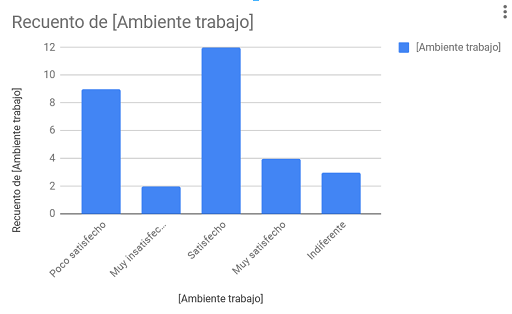
\includegraphics[width=1\textwidth]{graficoambiente}
	\captionof{figure}{La gráfica representa el grado de satisfacción en relación al ambiente de trabajo}
\end{center}

\begin{center}
	\centering
	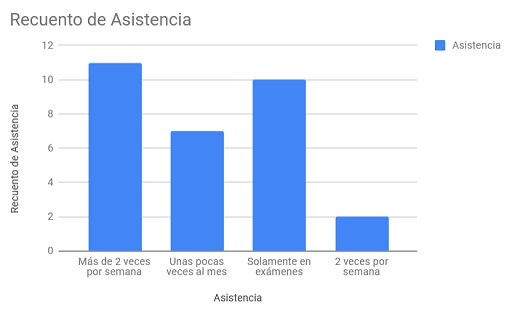
\includegraphics[width=1\textwidth]{graficoasistencia}
	\captionof{figure}{La gráfica refleja la asiduidad que tienen usuarios en relación al uso de la biblioteca}
\end{center}

\begin{center}
	\centering
	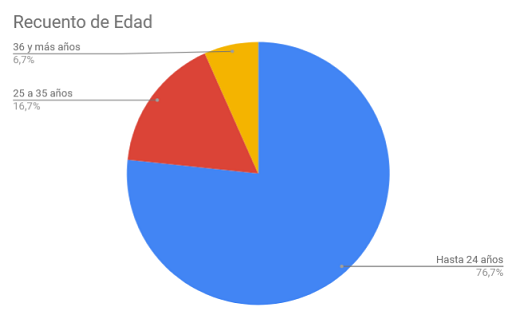
\includegraphics[width=1\textwidth]{graficoedad}
	\captionof{figure}{La gráfica refleja la proporción de género entre los usuarios encuestados}
\end{center}
\begin{center}
	\centering
	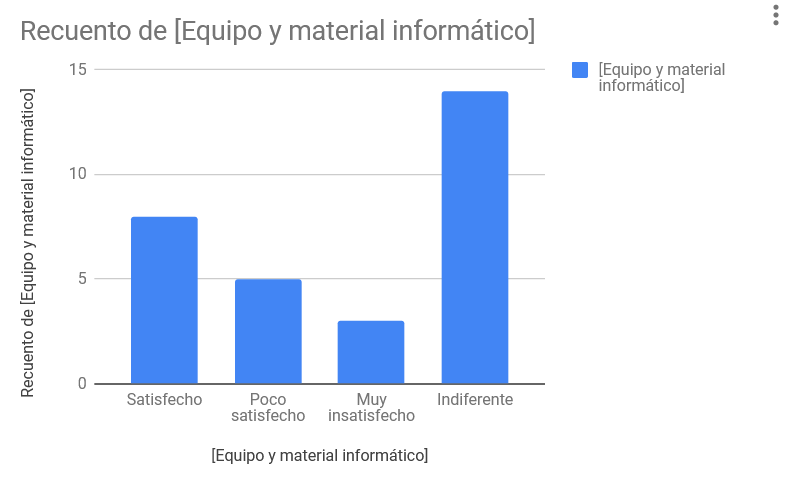
\includegraphics[width=1\textwidth]{graficoeqInformatico}
	\captionof{figure}{La gráfica refleja el grado de satisfacción que tienen los usuarios en relación al material informático disponible en la biblioteca}
\end{center}
\begin{center}
	\centering
	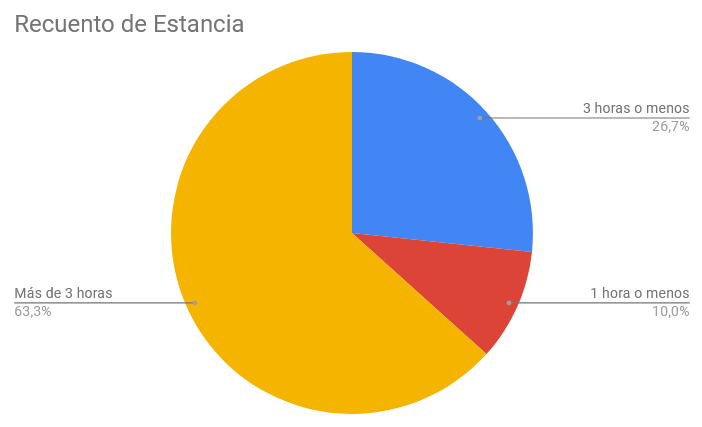
\includegraphics[width=1\textwidth]{graficoestancia}
	\captionof{figure}{La gráfica indica el tiempo que permanecen los usuarios en la bibliteca}
\end{center}\begin{center}
	\centering
	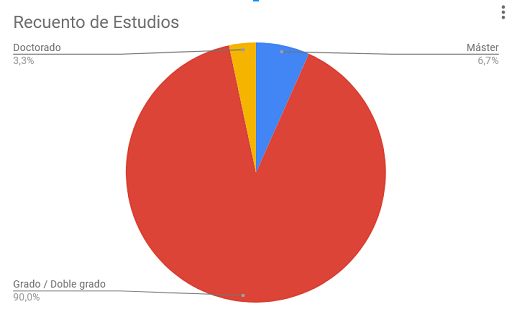
\includegraphics[width=1\textwidth]{graficoestudios}
	\captionof{figure}{La gráfica indica el nivel de estudios que tienen los usuarios que hacen uso de la biblioteca}
\end{center}\begin{center}
	\centering
	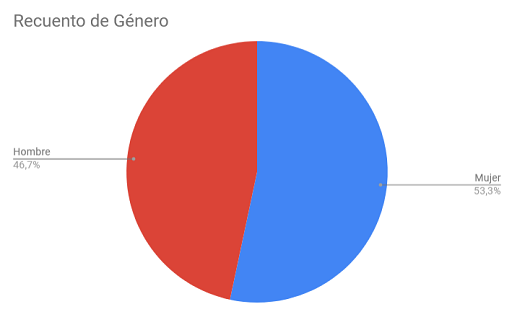
\includegraphics[width=1\textwidth]{graficogenero}
	\captionof{figure}{Esta gráfica refleja la proporción de género entre los usuarios encuestados.\\\\}
\end{center}\begin{center}
	\centering
	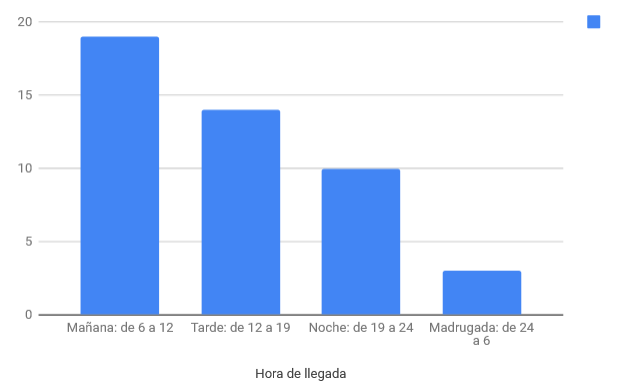
\includegraphics[width=1\textwidth]{graficohora_llegada}
	\captionof{figure}{La gráfica representa el tramo de horario de llegada donde se concentra el mayor o menor número de usuarios}
\end{center}\begin{center}
	\centering
	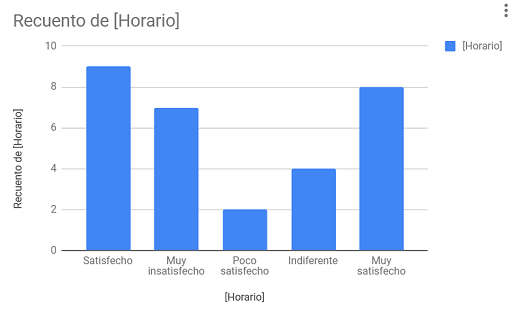
\includegraphics[width=1\textwidth]{graficohorario}
	\captionof{figure}{La gráfica representa el grado de satisfacción en relación al horario disponible que tiene la biblioteca}
\end{center}\begin{center}
	\centering
	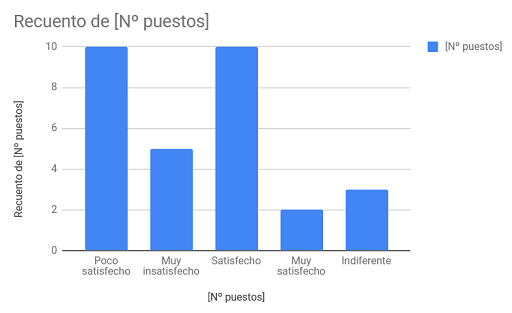
\includegraphics[width=1\textwidth]{graficonpuestos}
	\captionof{figure}{La gráfica representa el grado de satisfacción en relación a la cantidad de número de puestos existentes en la biblioteca}
\end{center}\begin{center}
	\centering
	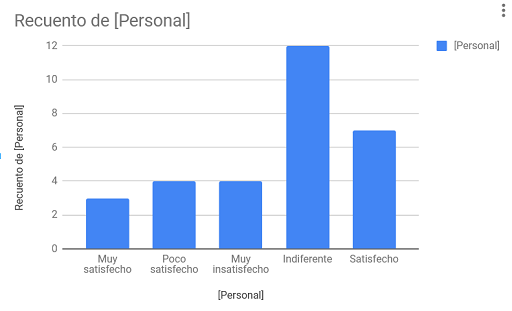
\includegraphics[width=1\textwidth]{graficopersonal}
	\captionof{figure}{La gráfica representa el grado de satisfacción en relación al trato que tienen los usuarios con el personal de la biblioteca}
\end{center}\begin{center}
	\centering
	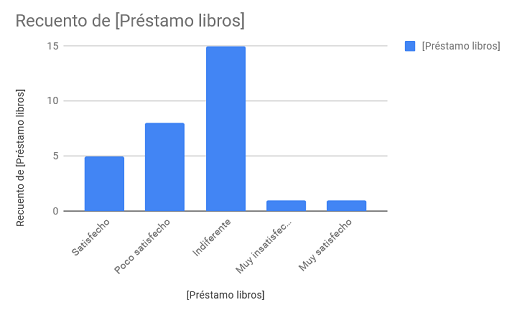
\includegraphics[width=1\textwidth]{graficoprestamo}
	\captionof{figure}{La gráfica representa el grado de satisfacción en relación al préstamo de libros}
\end{center}\begin{center}
	\centering
	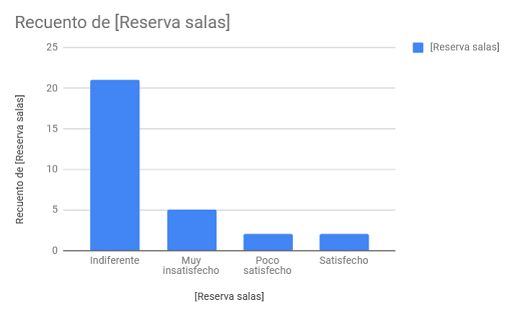
\includegraphics[width=1\textwidth]{graficoreserva}
	\captionof{figure}{La gráfica representa el grado de satisfacción en relación a la reserva de las salas de estudio}
\end{center}\begin{center}
	\centering
	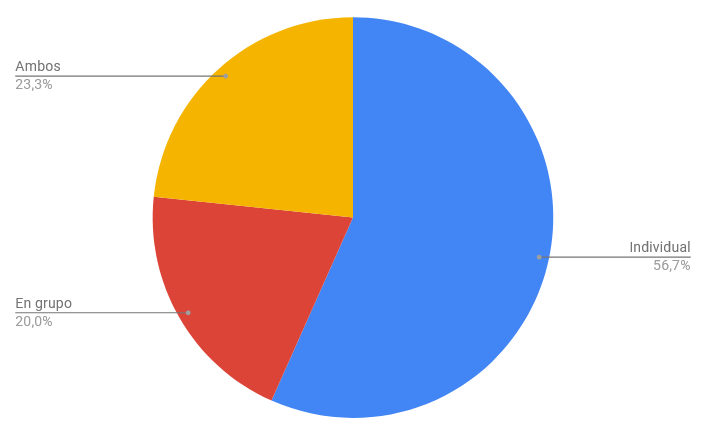
\includegraphics[width=1\textwidth]{graficouso}
	\captionof{figure}{La gráfica refleja el tipo de uso que los usuarios emplean al estudiar}
\end{center}

\subsection{Conclusiones de la encuesta}

	Hemos reunido la opinión de varias personas las cuales quedan repartidas equitativamente entre los distintos grados del nivel de estudios; donde hemos puesto nuestro enfoque.\\

	De las respuestas podemos concluir los siguientes datos relevantes en relación a los usuarios y al uso de la biblioteca:
\begin{itemize}

\item El horario de llegada. Es importante porque la información que nos proporciona es saber el tramo de horario en donde los usuarios usan más o menos la biblioteca.\\

\item El nivel de estudios. Este dato es importante porque la información que nos proporciona es saber el tipo de nivel cultural a tratar.\\

\item El tiempo de uso. Nos proporciona información en relación al tiempo que utilizan los usuarios la biblioteca en su mayoría.\\

\item La forma de estudio (individual,en grupo o ambas). Esta información es relevante para emplear una distribución eficiente para el uso de los usuarios.\\

\end{itemize}


\section{Estudio de la competencia} %%competencia total, parcial.\\\\.\\\\.\\


\subsection{Criterio de selección} %%?????

\subsection{Criterio de evaluación} %%??????

\subsection{Aplicaciones analizadas} %%TABLAS


\section{Lista de factoides}

\begin{itemize}
\item \textbf{Factoides de cuestionarios}
\begin{itemize}
\item Nuestros usuarios son mayoritariamente hombres y mujeres jóvenes (menores de 24 años) que estudian un grado/doble grado.\\

\item Aproximadamente, hay tantos usuarios hombre como mujer.\\

\item El 76.\\7\% de los usuarios son menores de 24 años, un 16.\\7\% tienen entre 25 y 35 años, el 6.\\7\% restante son usuarios con 36 o más años.\\

\item El 90\% de los usuarios estudian un grado/doble grado, el 6.\\7\% de ellos estudia un máster y el 3.\\3\% estudian un doctorado.\\

\item El 56.\\7\% de los usuarios acuden para estudiar de forma individual, mientras que un 20\% de ellos trabajan en grupo y el 23.\\3\% restante estudian tanto de forma individual como en grupo.\\

\item Los usuarios que trabajan de forma individual en algunos casos pueden llegar a representar el 80\% de los usuarios.\\

\item Los estudiantes de máster y doctorado permanecen durante largos periodos de tiempo en la biblioteca.\\

\item Por lo general los usuarios de grado/doble grado asisten por la mañana y permanecen más de 3 horas.\\

\item Un 70\% de los usuarios no tiene una opinión sobre la reserva de salas para trabajar en grupo.\\

\item Respecto al préstamo de libros un 50\% de los usuarios no los toma prestados, mientras que un 60\% de los usuarios que si reservan no se encuentran satisfechos.\\

\item Un 50\% de los usuarios no están satisfechos con el número de puestos físicos de la biblioteca

\item Un 36\% de los usuarios no están a gusto con el ambiente de trabajo.\\

\item Los usuarios que han valorado positivamente el horario de la biblioteca son usuarios que permanecen largos periodos de tiempo de forma individual en la misma.\\

\item Por lo general los usuarios están conformes con el personal de la biblioteca.\\

\item Los usuarios utilizan poco el equipo y material informático; al menos un gran número de usuarios encuestados parece indiferente y poco satisfecho.\\

\item Los usuarios que asisten a la biblioteca 2 o más veces por semana son mayoritariamente mujeres (69\%).\\ 

\item Los usuarios que asisten a la biblioteca con poca frecuencia o solamente en periodo de exámenes son mayoritariamente hombres (58\%).\\

\item Las mujeres permanecen más tiempo en la biblioteca que los hombres.\\

\item Los usuarios que estudian en grupo no están satisfechos con la reserva de salas.\\
\end{itemize}




\item \textbf{Factoides de la competencia}
\begin{itemize}

\item Todas las aplicaciones cuentan con un mapa de la zona y la localización de las salas.\\

\item Nuestra aplicación solamente funciona en plataformas móviles.\\

\item Nuestra aplicación es la única que es Open Source en su plataforma.\\

\item Solamente Worldshare y nuestra aplicación son Open Source.\\

\item Las pantallas de los laboratorios ofrecen tanta información acerca de los asientos como la nuestra.\\

\item Yelmo cines y la aplicación de los puestos de laboratorio muestran el estado actual de las salas.\\
\item La mayoría de aplicaciones son multiplataforma y casi todas funcionan para dispositivos móviles.\\
CISNE y Worldshare tienen página web.\\


\end{itemize}
\end{itemize}


Factoides relativos a aspectos generales de la aplicación y su contenido:




Factoides relativos a las estadisticas:











\end{document}

%COMENTAARIOS
% \todo[inline, color=green!40]{EJEMPLO DE COMENTARIO}

% PARA INCLUIR UNA FOTOGRAFIA:
%\begin{figure}
%\centering
%\includegraphics[width=0.\\5\textwidth]{~/DIRECCION/A/IMAGEN.\\jpg}
%\caption{\label{fig:imagen}DESCRIPCION.\\}
%\end{figure}

% \dots

% ENUMERACION:
%\begin{enumerate}
%\item Enumeracion 1
%\item Enumeracion 2
%\end{enumerate}

%\begin{itemize}
%\item PUNTO 1

% PARA INCLUIR UNA TABLA:
%\begin{table}[h] %LA h PARA INDICAR QUE LA TABLA NO SEA FLOATING
%\centering
%\begin{tabular}{l|r}
%Fila 0 \\\hline
%Fila 1 & Contenido 1 \\
%Fila 2 & Contenido 2
%\end{tabular}
%\caption{\label{tab:widgets}Ejemplo de tabla.\\}
%\end{table}

%\item PUNTO 2
%\end{itemize}

%\bibliography{BIBLIOGRAFIA}


